\chapter{Estimation of diffusion coefficients in rat cardiomyocytes}
\label{ch:exp_res}
\section{Cardiomyocyte preparation}
\lettrine[lines=2, lhang=0.33, loversize=0.25]{N}
{either of the dyes used} in this work (\ATP\ and \DEX ) are able to permeate the cell
membrane. This can be seen on \F{\ref{fig:cells_1}}, where, contrary
to the fluorescent signal from the membrane permeable form of
Mitotracker Green dye (\F{\ref{fig:cells_1}A}), \ATP\ is not
able to pass into the cytosol (\F{\ref{fig:cells_1}B}). In order to use \ac{RICS} to estimate the \ac{DC}s of these
dyes, they have to be allowed to enter into the cell. This can be
achieved through saponin permeabilization of the cell membrane
\cite{Vendelin_08_AmJPhysiolCellPhysiol_295_pC1302}. Initially, saponin
permeabilization was used also in this work, but it
became evident that exposure to saponin resulted in the cells
hypercontracting within a few hours. The full protocol for \ac{RICS} measurements, however,
takes several hours to complete. This necessitated the need to come up with
an alternative method of introducing the dyes into the cell. 
\begin{figure}[h!]
  \centering
    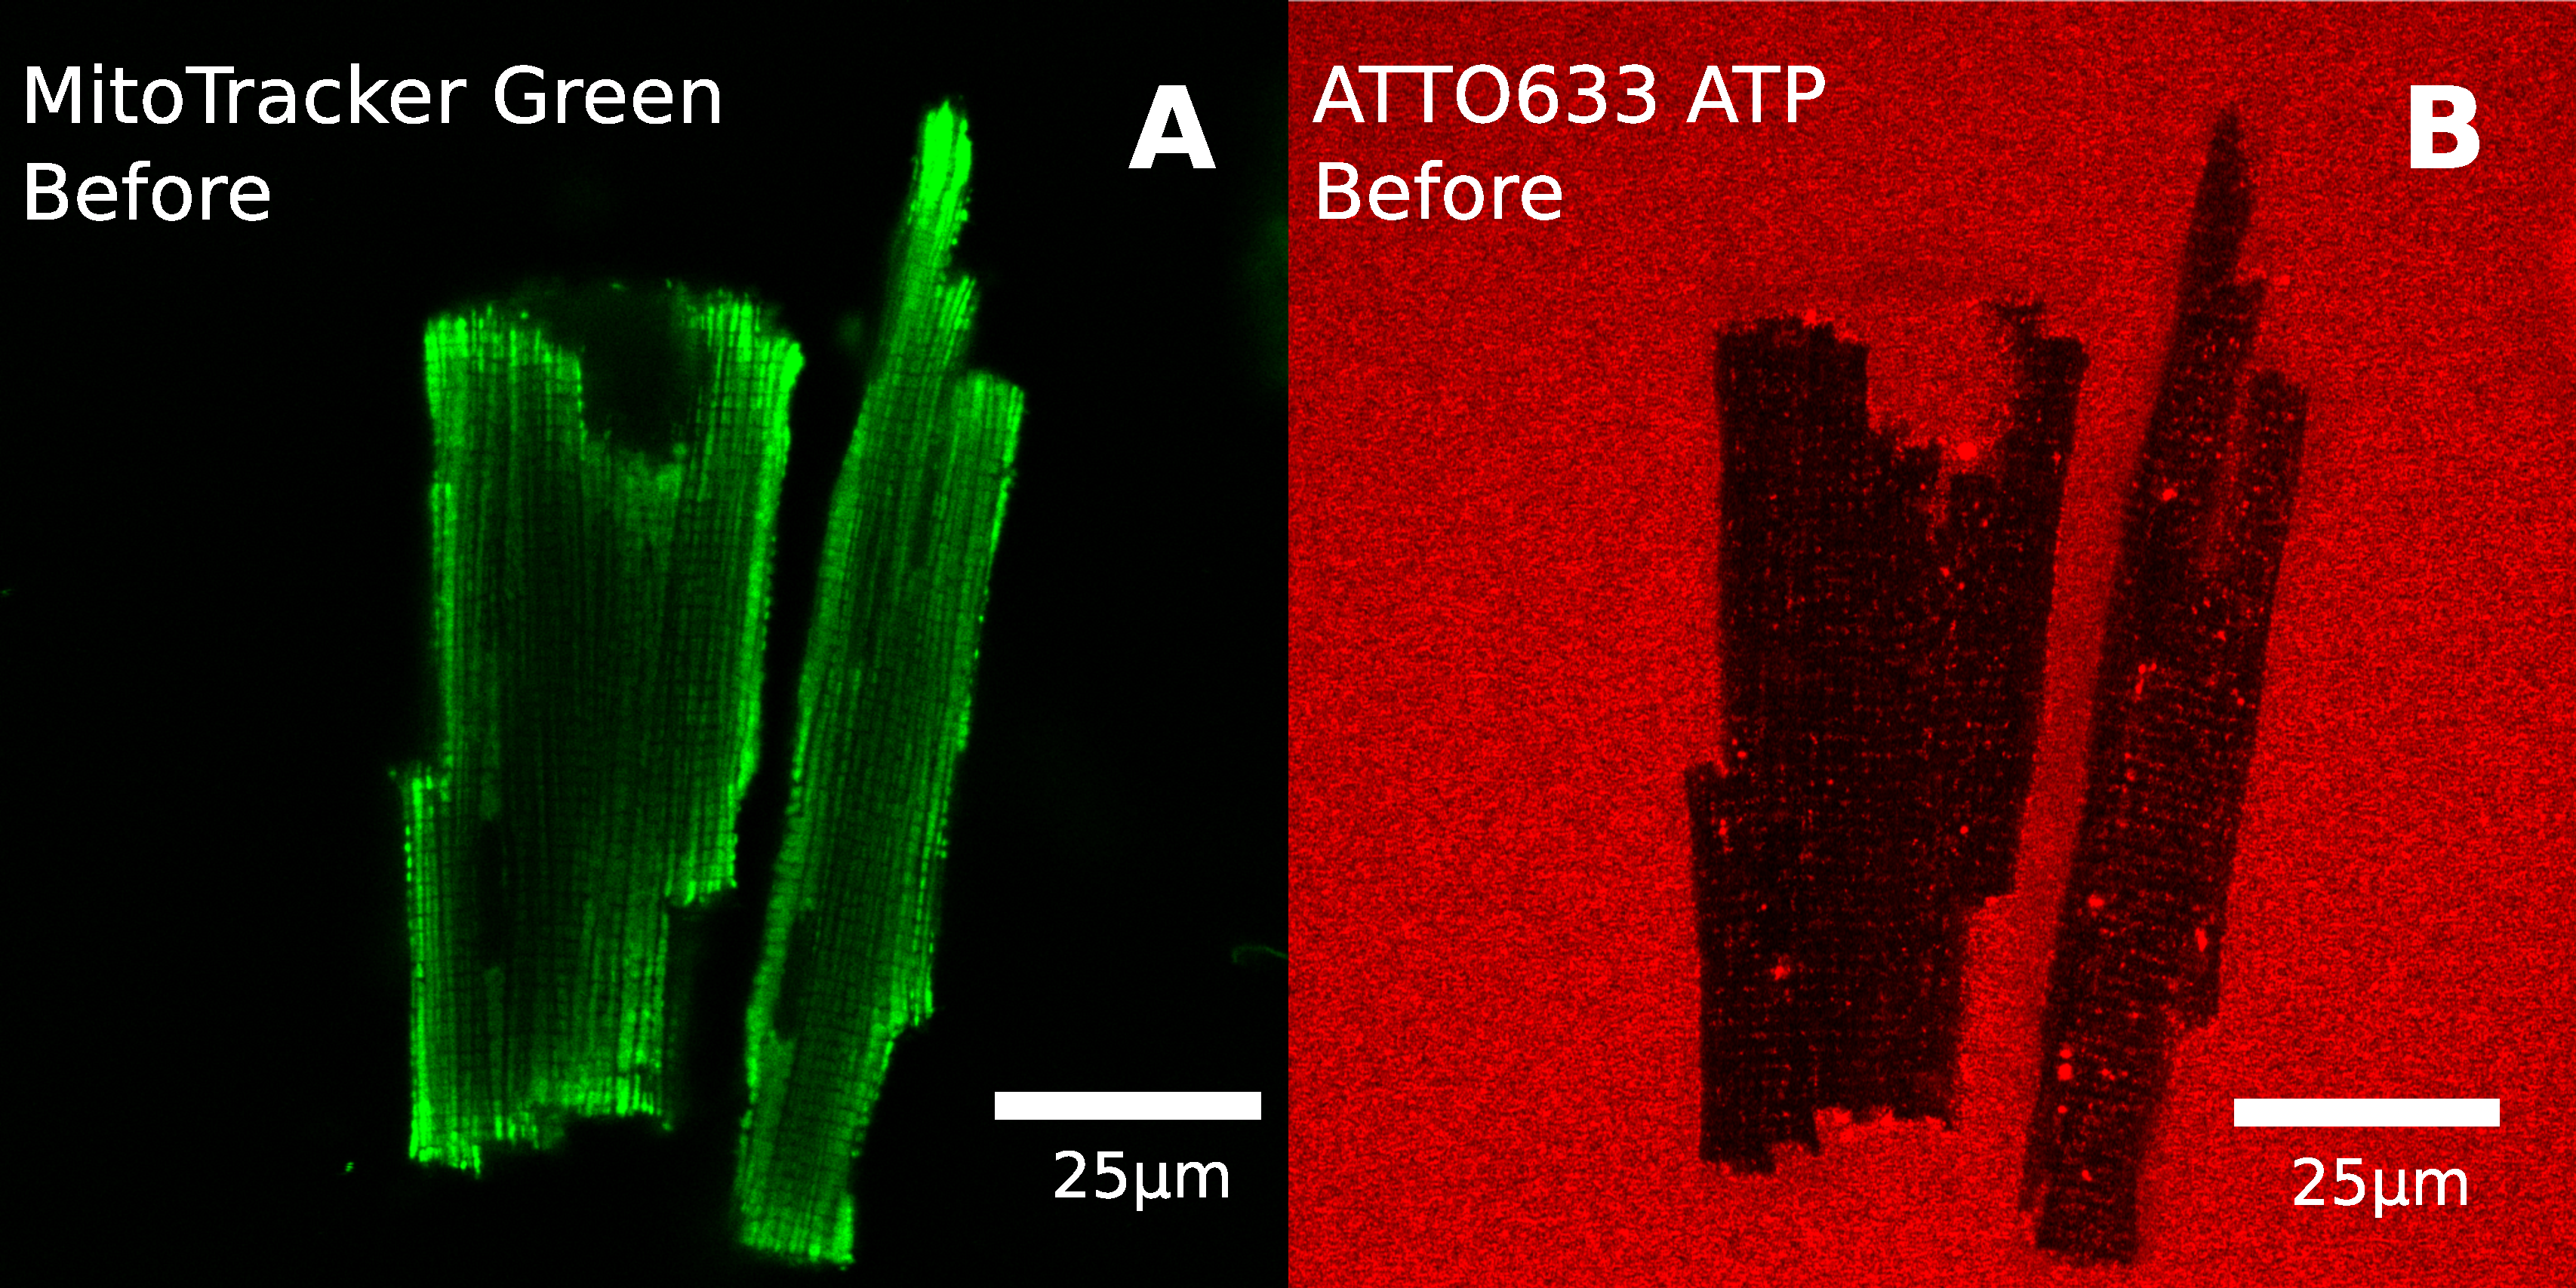
\includegraphics[width=10cm]{figures/cells1.pdf}
    \caption[Non-permeated cardiomyocytes]{Confocal images of rat
    cardiomyocytes in measurement solution. On the left image (A)
    membrane permeable Mitotracker Green dye has permeated the membrane and accumulates in the cell. On the right image (B) \ATP\ is visible in the solution
    outside the cell and is not able to enter the cytosol.}
  \label{fig:cells_1}
%The autocorrelation at shift vector $\Delta \mathbf{h}=(\xi,\psi)$ for an image with
%fluorescence values $F(\mathbf{p})$ at location $\mathbf{p} = (x,y)$ is given by:
%{\small
\end{figure}
\begin{figure}[t]
  \centering
    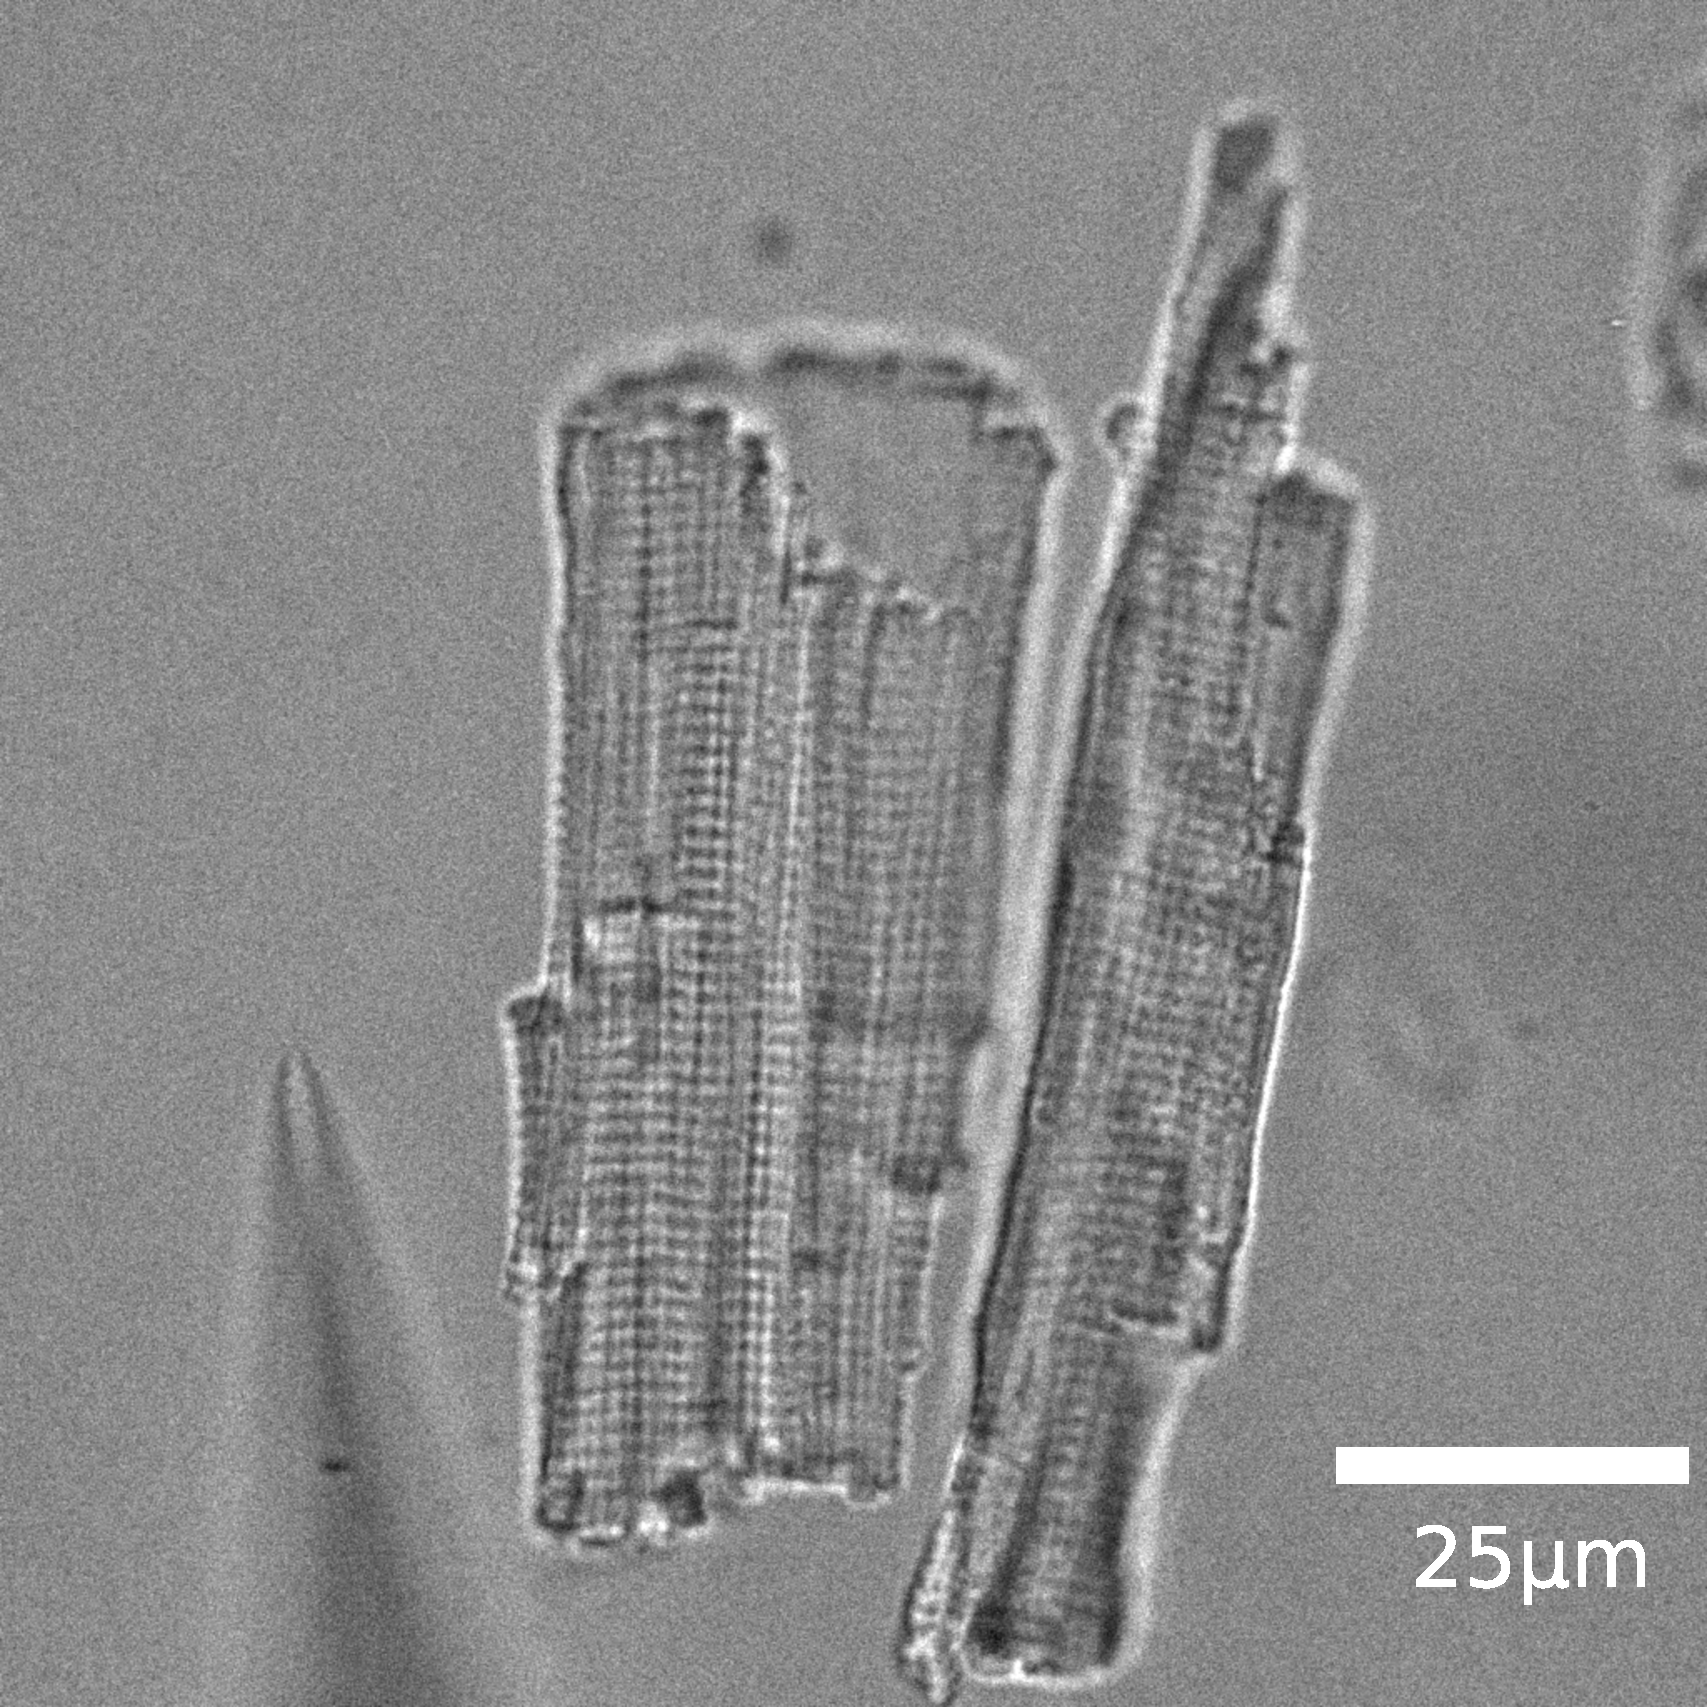
\includegraphics[width=5cm]{figures/cells2.pdf}
    \caption[Permeation of cardiomyocytes]{The cell membrane is permeated mechanically with a
    glass pipette (tip $\diameter 0.5$ $\mu$m). Both the pipette and the
    cell are shown on this transmission image.}
  \label{fig:cells_2}
%The autocorrelation at shift vector $\Delta \mathbf{h}=(\xi,\psi)$ for an image with
%fluorescence values $F(\mathbf{p})$ at location $\mathbf{p} = (x,y)$ is given by:
%{\small
\end{figure}

In this work, viable permeabilized cells were obtained by using a glass pipette with a diameter of $0.5$ $\mu$m to mechanically
``poke'' 2-3 holes into the cell membrane (\F{\ref{fig:cells_1}}).
Within minutes after completing this procedure, fluorescence signal from \ATP\
could be recorded from withing the cell. After this the full \ac{RICS}
protocol was carried out. Compared to saponin permeabilization, the
viability of the ``poked'' cells was increased by several hours.

\begin{figure}[t!]
  \centering
    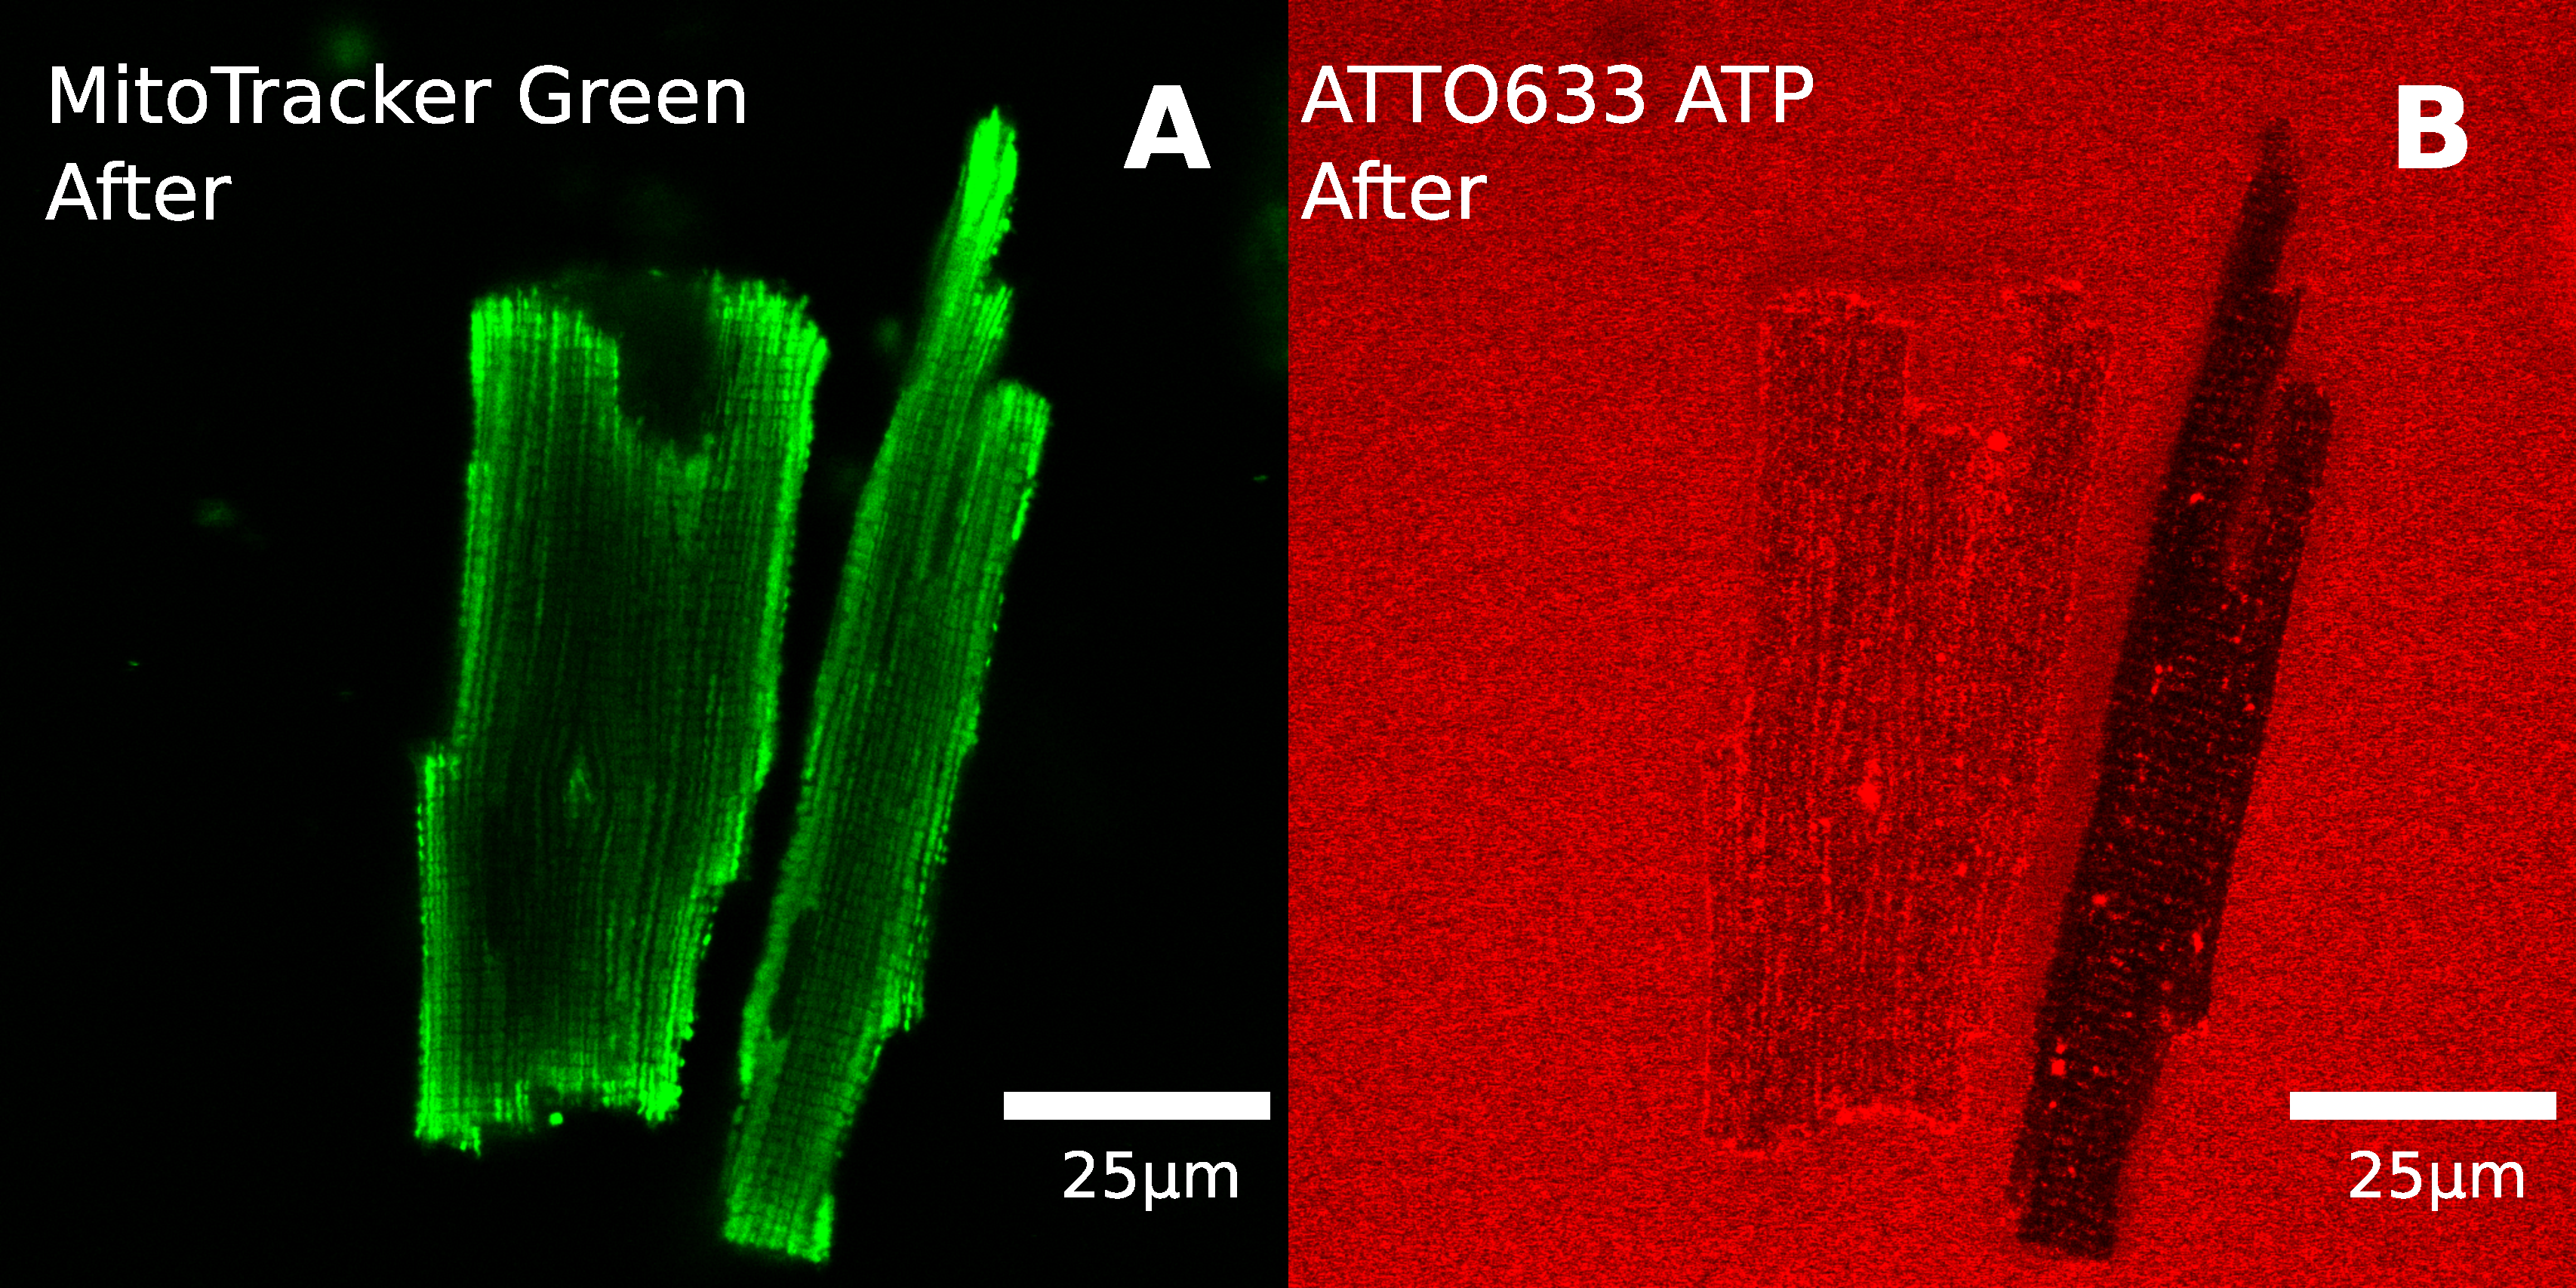
\includegraphics[width=10cm]{figures/cells3.pdf}
    \caption[Permeated cardiomyocytes]{Confocal images of cardiomyocytes after ``poking''.
    The Mitotracker Green signal is unaltered (A) but fluorescence from \ATP\ is now
    visible in the cytosol.}
  \label{fig:cells_3}
%The autocorrelation at shift vector $\Delta \mathbf{h}=(\xi,\psi)$ for an image with
%fluorescence values $F(\mathbf{p})$ at location $\mathbf{p} = (x,y)$ is given by:
%{\small
\end{figure}
%%\caption{Diffusion constants (D$_{TR}$ and D$_L$ in transverse and
%  longitudinal directions, respectively) obtained from raster image
%  correlation spectroscopy at 26$^\circ$C. Listed values were
%  obtained in water, measurement solution (solution), or \ac{CM} s. On the
%  basis of $n$ experiments, several parameters were determined in
%  addition to diffusion coefficient(s): concentration, triplet time
%  constant $\tau$ and triplet state contribution $T$. Correlations
%  between fluctuation of fluorescence signal were fitted by isotropic
%  model (diffusion coefficient specified only as D$_{TR}$),
%  anisotropic model (D$_{TR}$ and D$_L$ specified), or model with two
%  components (Cmp). }
  \begin{tabular}{llccc}
\hline
&   & \multicolumn{3}{c}{Diffusion}  \\
\multicolumn{1}{c}{Dye} & \multicolumn{1}{c}{Media} &
 Cmp.  & \multicolumn{1}{c}{D$_{TR}$} &
\multicolumn{1}{c}{D$_L$} \\
 & & &
 \multicolumn{1}{c}{$\mu m^2/s$} & \multicolumn{1}{c}{$\mu m^2/s$} \\
\hline
\\ 
 %& water &  & \texttt{442$\pm$4} & \texttt{483$\pm$7}  \\
% & solution &  & {362$\pm$4} &  \\
 %& solution &  & \texttt{348$\pm$2} & \texttt{403$\pm$10}\\
\\ ATTO633-ATP & water &  & {326$\pm$13} & \\
 %& water &  & \texttt{322$\pm$15} & \texttt{337$\pm$12}\\
 & solution &  & {195$\pm$8}&   \\
 %& solution &  & \texttt{183$\pm$11} & \texttt{222$\pm$3}\\
 %& \ac{CM}\ &  & \texttt{4.0$\pm$0.6} & \texttt{4.6$\pm$0.9}\\
 %& \multirow{2}{*}{\ac{CM}} & \multirow{2}{*}{}
 %&\multirow{2}{*}{$\Big\{\Big.\;$$\begin{matrix}\mathtt{1}\\\mathtt{2}\end{matrix}$}& &
 %\texttt{0.7$\pm$0.3} & \texttt{0.8$\pm$0.2} &
 %\multirow{2}{*}{$\Big.\Big\}$} &
 %\multirow{2}{*}{}\\
 &\multirow{2}{*}{\ac{CM}}   &1 & {0.7$\pm$0.3} &
 {0.8$\pm$0.2}\\
 &   &2 & {24$\pm$6} & {35$\pm$8}\\
\\ Alexa647-dextran10K & water &  & {62$\pm$1}& \\
 %& water &   & \texttt{60$\pm$2} & \texttt{65$\pm$2}\\
 & solution &   & {53$\pm$1}&   \\
 %& solution &   & \texttt{51$\pm$2} & \texttt{57$\pm$1}\\
 & \ac{CM}\ &   & {16$\pm$2} & {19$\pm$3}
 \\
ATTO655-COOH & water &  & {454$\pm$3} &  \\
% & \ac{CM} (saponin)\ & 7 && \texttt{20$\pm$6} & \texttt{15$\pm$2} & \texttt{19$\pm$1} & \texttt{0.28$\pm$0.04} & \texttt{5.1$\pm$1.8}\\

\end{tabular}


\section{Diffusion coefficients in cardiomyocytes}
Diffusion coefficient estimates were obtained by fitting the
experimentally calculated \ac{CF} with the theoretical
\ac{CF} from \Eq{~\ref{eq:G_2ctrip}} as explained in detail in \PaperIII.  A summary of the results
obtained is presented in Table \ref{table:exp_res}. The table with full
experimental results is given in \PaperIII. The two \acp{DC} shown for
\ATP\ in \ac{CM} are the slow and freely diffusing forms of the dye.
Separating \ATP\ into two subspecies was necessary due to \ATP\ probably
binding to some intracellular proteins and thereby creating a second,
slower diffusing form of \ATP. For \DEX\ a second component was not necessary.

Also shown, are results for a third dye (Atto655-COOH) diffusing in
water. The \ac{DC} of this dye has been determined in water
\cite{Muller_08_EPL_EurophysicsLetters__83_p46001}, allowing us to use
this data to test the accuracy of our method. Our estimate of 454$\pm$3 $\mu$m$^2$/s obtained
at 26$^\circ$ is in good agreement with published data for Atto655-COOH:
426$\pm$6 $\mu$m$^2$/s obtained at 25$^\circ$
\cite{Muller_08_EPL_EurophysicsLetters__83_p46001} after correcting for
the temperature difference. 

On \F{\ref{fig:d_atto_dex}} results for \ATP\ and \DEX\ are presented
graphically. From here the effect of anisotropy of diffusion and the
reduction experienced by \ATP\ and \DEX\ can be seen. 
\begin{table}
\begin{center}
    \begin{small}
%\caption{Diffusion constants (D$_{TR}$ and D$_L$ in transverse and
%  longitudinal directions, respectively) obtained from raster image
%  correlation spectroscopy at 26$^\circ$C. Listed values were
%  obtained in water, measurement solution (solution), or \ac{CM} s. On the
%  basis of $n$ experiments, several parameters were determined in
%  addition to diffusion coefficient(s): concentration, triplet time
%  constant $\tau$ and triplet state contribution $T$. Correlations
%  between fluctuation of fluorescence signal were fitted by isotropic
%  model (diffusion coefficient specified only as D$_{TR}$),
%  anisotropic model (D$_{TR}$ and D$_L$ specified), or model with two
%  components (Cmp). }
  \begin{tabular}{llccc}
\hline
&   & \multicolumn{3}{c}{Diffusion}  \\
\multicolumn{1}{c}{Dye} & \multicolumn{1}{c}{Media} &
 Cmp.  & \multicolumn{1}{c}{D$_{TR}$} &
\multicolumn{1}{c}{D$_L$} \\
 & & &
 \multicolumn{1}{c}{$\mu m^2/s$} & \multicolumn{1}{c}{$\mu m^2/s$} \\
\hline
\\ 
 %& water &  & \texttt{442$\pm$4} & \texttt{483$\pm$7}  \\
% & solution &  & {362$\pm$4} &  \\
 %& solution &  & \texttt{348$\pm$2} & \texttt{403$\pm$10}\\
\\ ATTO633-ATP & water &  & {326$\pm$13} & \\
 %& water &  & \texttt{322$\pm$15} & \texttt{337$\pm$12}\\
 & solution &  & {195$\pm$8}&   \\
 %& solution &  & \texttt{183$\pm$11} & \texttt{222$\pm$3}\\
 %& \ac{CM}\ &  & \texttt{4.0$\pm$0.6} & \texttt{4.6$\pm$0.9}\\
 %& \multirow{2}{*}{\ac{CM}} & \multirow{2}{*}{}
 %&\multirow{2}{*}{$\Big\{\Big.\;$$\begin{matrix}\mathtt{1}\\\mathtt{2}\end{matrix}$}& &
 %\texttt{0.7$\pm$0.3} & \texttt{0.8$\pm$0.2} &
 %\multirow{2}{*}{$\Big.\Big\}$} &
 %\multirow{2}{*}{}\\
 &\multirow{2}{*}{\ac{CM}}   &1 & {0.7$\pm$0.3} &
 {0.8$\pm$0.2}\\
 &   &2 & {24$\pm$6} & {35$\pm$8}\\
\\ Alexa647-dextran10K & water &  & {62$\pm$1}& \\
 %& water &   & \texttt{60$\pm$2} & \texttt{65$\pm$2}\\
 & solution &   & {53$\pm$1}&   \\
 %& solution &   & \texttt{51$\pm$2} & \texttt{57$\pm$1}\\
 & \ac{CM}\ &   & {16$\pm$2} & {19$\pm$3}
 \\
ATTO655-COOH & water &  & {454$\pm$3} &  \\
% & \ac{CM} (saponin)\ & 7 && \texttt{20$\pm$6} & \texttt{15$\pm$2} & \texttt{19$\pm$1} & \texttt{0.28$\pm$0.04} & \texttt{5.1$\pm$1.8}\\

\end{tabular}


\end{small}
\caption[Experimental \acl{DC} values for \ATP\ and \DEX]{Diffusion coefficient values for \ATP\ and \DEX\ in water,
solution and cardiomyocyte. In case of anisotropic diffusion, \ac{DC}
values for both transverse(TR) and longitudinal(L) directions are
given (\ac{DC} in the $z$ direction is assumed equal to the \ac{DC} in $x$
direction). For isotropic diffusion only one \ac{DC} is shown which applies
for all directions. Data shown is mean $\pm$ standard deviation. }
\label{table:exp_res}
\end{center}
\end{table}

\begin{figure}
  \centering
    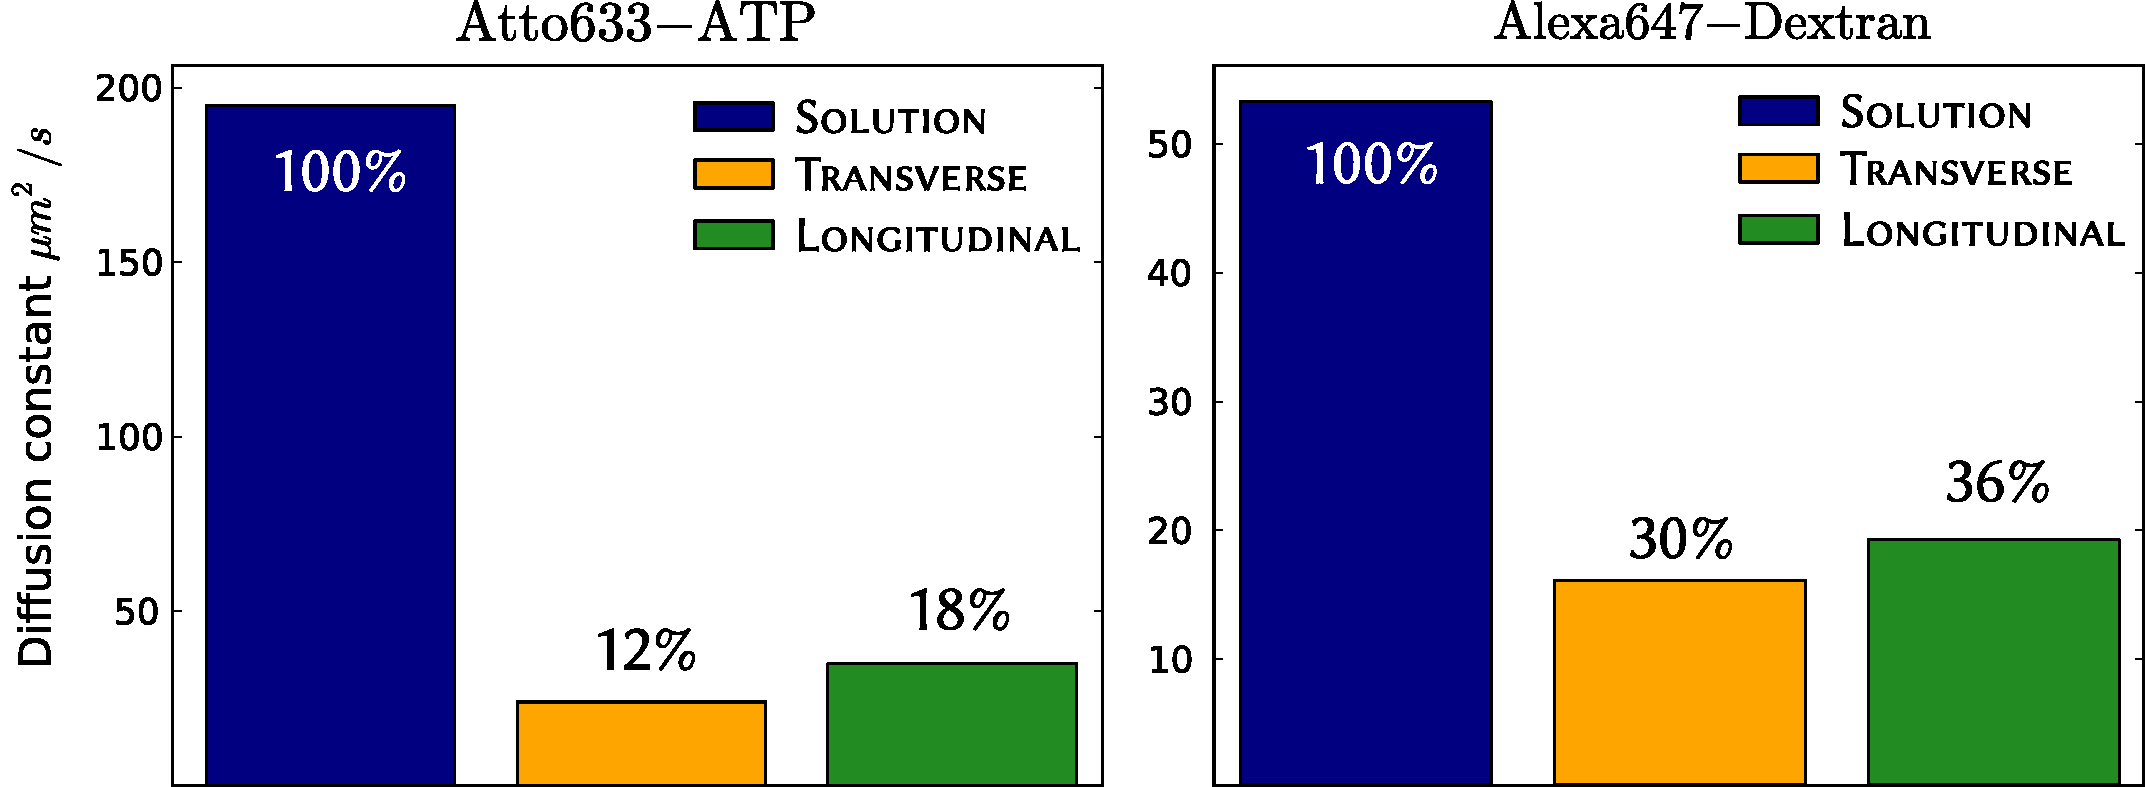
\includegraphics[width=12cm]{figures/d_atto_dex.pdf}
    \caption[Diffusion coefficients of \ATP\ and \DEX\ in solution and
    cardiomyocyte]{Diffusion coefficients of \ATP\ and \DEX in solution and
    cardiomyocyte. The percentages show the \acp{DC} relative to \ac{DC}
    in solution.}
  \label{fig:d_atto_dex}
%The autocorrelation at shift vector $\Delta \mathbf{h}=(\xi,\psi)$ for an image with
%fluorescence values $F(\mathbf{p})$ at location $\mathbf{p} = (x,y)$ is given by:
%{\small
\end{figure}
\begin{figure}[b!]
  \centering
    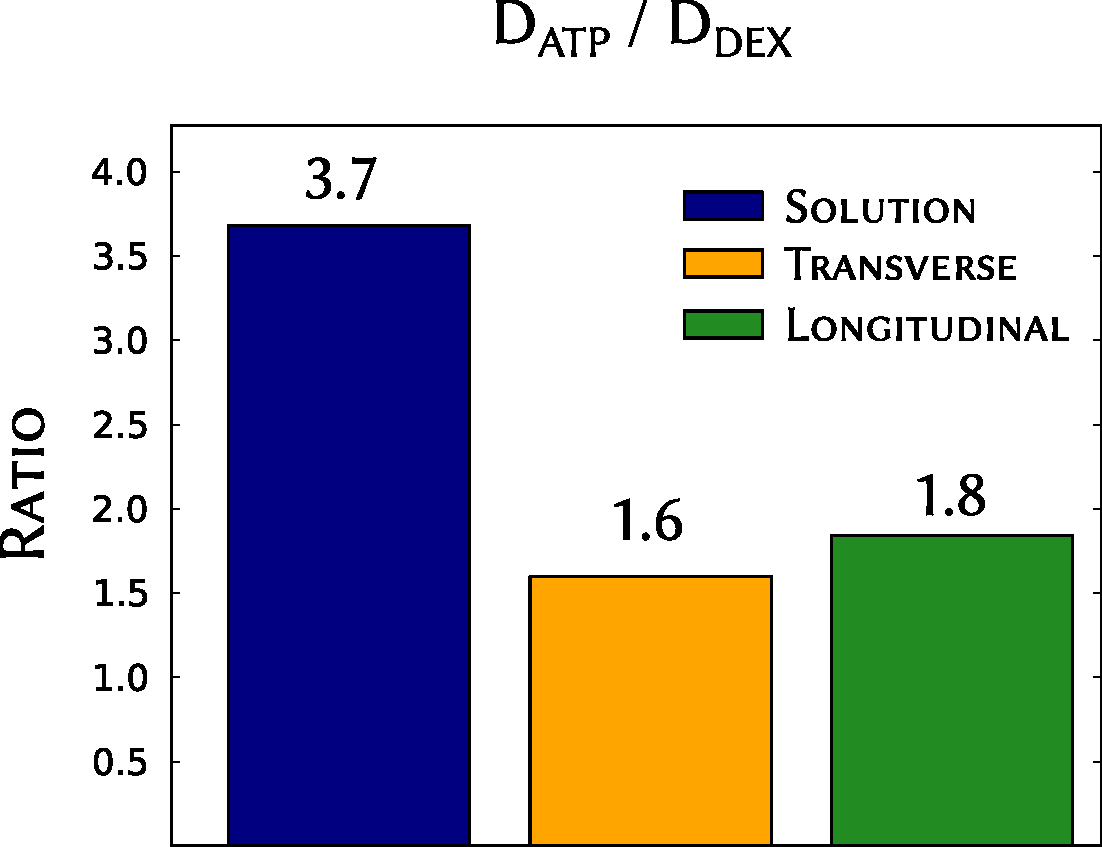
\includegraphics[width=6cm]{figures/ratio.pdf}
    \caption[Ratio of \aclp{DC} of \ATP\ and \DEX]{Ratio of \acp{DC} of
    \ATP\ and \DEX\ in solution and in the transverse and longitudinal
    directions of the cell.}
  \label{fig:ratio}
%The autocorrelation at shift vector $\Delta \mathbf{h}=(\xi,\psi)$ for an image with
%fluorescence values $F(\mathbf{p})$ at location $\mathbf{p} = (x,y)$ is given by:
%{\small
\end{figure}
\section{Conclusions}
The most striking result of this study is the fact that the \ac{DC} of
\ATP\ is reduced more than that of \DEX\ when comparing diffusion in
\ac{CM} and solution. This is visualized in \F{\ref{fig:ratio}} where the
ratio of \ac{DC} of \ATP\ to that of \DEX\ is shown. As can be seen, the more
than 3 time difference in solution is reduced to less than 2 in the
cytoplasm, indicating that the diffusion of the smaller molecule (\ATP)
is hindered more than that of the larger one (\DEX). This is unexpected,
as relative decrease of \ac{DC} is usually larger for
larger molecules \cite{Muramatsu_88_ProcNatlAcadSci_85_p2984}.

Secondly, longer viability of the cardiomyocytes during the duration of
the experimental protocol indicates that the employed ``poking''
technique is a good alternative to saponin permeabilization. The
drawback of the method is that it is time consuming and requires more
specialized equipment than is needed when using saponin permeabilization.
Furthermore, depending on how well the cells attach to the laminin
coated coverslip, several cells might need to be poked before the
procedure is successful and a permeated \ac{CM} is obtained for
performing \ac{RICS} measurements. A different approach of localized
permeabilization can be used as well. In this approach saponin is applied locally by a
micropipette in only one region of the cardiomyocyte
\cite{Abraham_02_JBiolChem_277_p24427}, whereby only a
section of the cell is exposed and permeabilized. However, this would
require extra equipment in addition to that used in the ``poking'' procedure. 

Lastly, increasing the amount of physical phenomena taken into account when deriving the
theoretical \acl{CF} increases the ability of the
theoretical fit to match experimental data. Addition of anisotropic
diffusion, two diffusing components of the same dye and triplet state
dynamics to the \ac{CF} as demonstrated in \ref{ch:rics} increases the ability
to produce consistent \ac{DC} estimations. Naturally, care has to be
taken to avoid overparameterizing the theoretical model used for fitting
experimental data. Additions to the theoretical \ac{CF} are made only in
cases when the physical process being observed warrants it. For example,
when fitting \DEX\ data from cardiomyocytes, a single component model is
used instead of a two component one, since the underlying physical process is deduced
to be of only one species of \DEX\ diffusing. 


